\documentclass{article}
\usepackage[utf8]{inputenc}
\usepackage[dvips]{graphicx}
\usepackage{a4wide}
\usepackage{amsmath}
\usepackage{euscript}
\usepackage{amssymb}
\usepackage{amsthm}
\usepackage{amsopn}
\usepackage{mathtools}
\usepackage{polynom}

\theoremstyle{definition}
\newtheorem*{definition}{Definition}
\newtheorem{theorem}{Theorem}
\newcommand{\cis}{\mbox{cis}}
\newcommand{\vv}{\ensuremath{\vec{v}}}
\newcommand{\vu}{\ensuremath{\vec{u}}}
\newcommand{\vw}{\ensuremath{\vec{w}}}
\newcommand{\vx}{\ensuremath{\vec{x}}}
\newcommand{\vy}{\ensuremath{\vec{y}}}
\newcommand{\vb}{\ensuremath{\vec{b}}}
\newcommand{\vo}{\ensuremath{\vec{0}}}
\newcommand{\va}{\ensuremath{\vec{a}}}
\newcommand{\ve}{\ensuremath{\vec{e}}}
\newcommand{\deriv}{\frac{d}{dz}}

\usepackage{halloweenmath, tikzsymbols}

\newcommand{\R}{\mathbb{R}}
\newcommand{\Z}{\mathbb{Z}}
\newcommand{\C}{\mathbb{C}}
\newcommand{\N}{\mathbb{N}}
\newcommand{\Q}{\mathbb{Q}}
\newcommand{\Arg}{\mbox{Arg}}
\newcommand{\Log}{\mbox{Log}}
\newcommand{\defn}{\fbox{definition}}
\newcommand{\thm}{\fbox{theorem}}
\newcommand{\infsum}{\sum_{n = 0}^{\infty}}
\newcommand{\pf}{\fbox{proof}}
\newcommand{\cor}{\fbox{corollary}}
\newcommand{\psum}{\sum_{n = 0}^N}
\newcommand{\prop}{\fbox{proposition}}


\newcommand{\cs}[1]{\color{blue}{#1}\normalcolor}
\newcommand{\ab}[1]{\color{red}{#1}\normalcolor}

\title{Complex Analysis}
\author{ajbergquist }
\date{August 2021}

\begin{document}
\fbox{problem 3} Find the taylor expansion of $1/z^2 = 1/2\frac{1}{1+(z-2)/2} = 1/2\frac{1}{1 - ((-1)(z-2))/2}$ about the point $z_0 = 2$. Then differentiate the series term by term to find the taylor expansion for $1/z^2$ about the same point.\\

\fbox{solution} First, note that $1/z^2$ is analytic everywhere inside the open circle for radius 2 centered at $z_0 = 2$. We know the taylor expansion for $1/(1-z) = \infsum z^n$, hence for $|z| < 1$, hence we can substitute $z$ for $(-1)\frac{z-2}{2}$ to find $1/2\frac{1}{1+(z-2)/2} = 1/2\infsum[(-1)^n((z-2)/2)^n = 1/2\infsum (-1)^n\big(\frac{z-2}{2}\big)^n.$ Differentiating term by term, multiplying both sides by $-1$, and translating the series backward by 1, we find $1/z^2 = -1/2\infsum (-1)^n(n)((z-2)/2)^{n-1}/2 = 1/4\sum_{n = 0}^\infty[(-1)^{n+1}= (-1)^{\cs{n}-1}](n)\big(\frac{z-2}{2}\big)^{n-1} = 1/4\infsum(-1)^n(n+1)\big(\frac{z-2}{2}\big)^n$.\\

\cs{Sec 72: 5/5}

\fbox{problem 4} Find the first four terms of the laurent series representation of $\frac{1}{e^z-1}$\\
\fbox{solution} First, we can apply the already known Maclaurin expansion of $e^z = \infsum z^n/n! = 1+z + z^2/2 + z^3/6 + z^4/24 + z^5/120 + z^6/720$, valid for all $z\in \C$. Hence, we can simply divide the sequences (this is nearly impossible to LaTex, so here's an image of it worked out until I find a way),
\begin{figure}[htbp]
\centerline{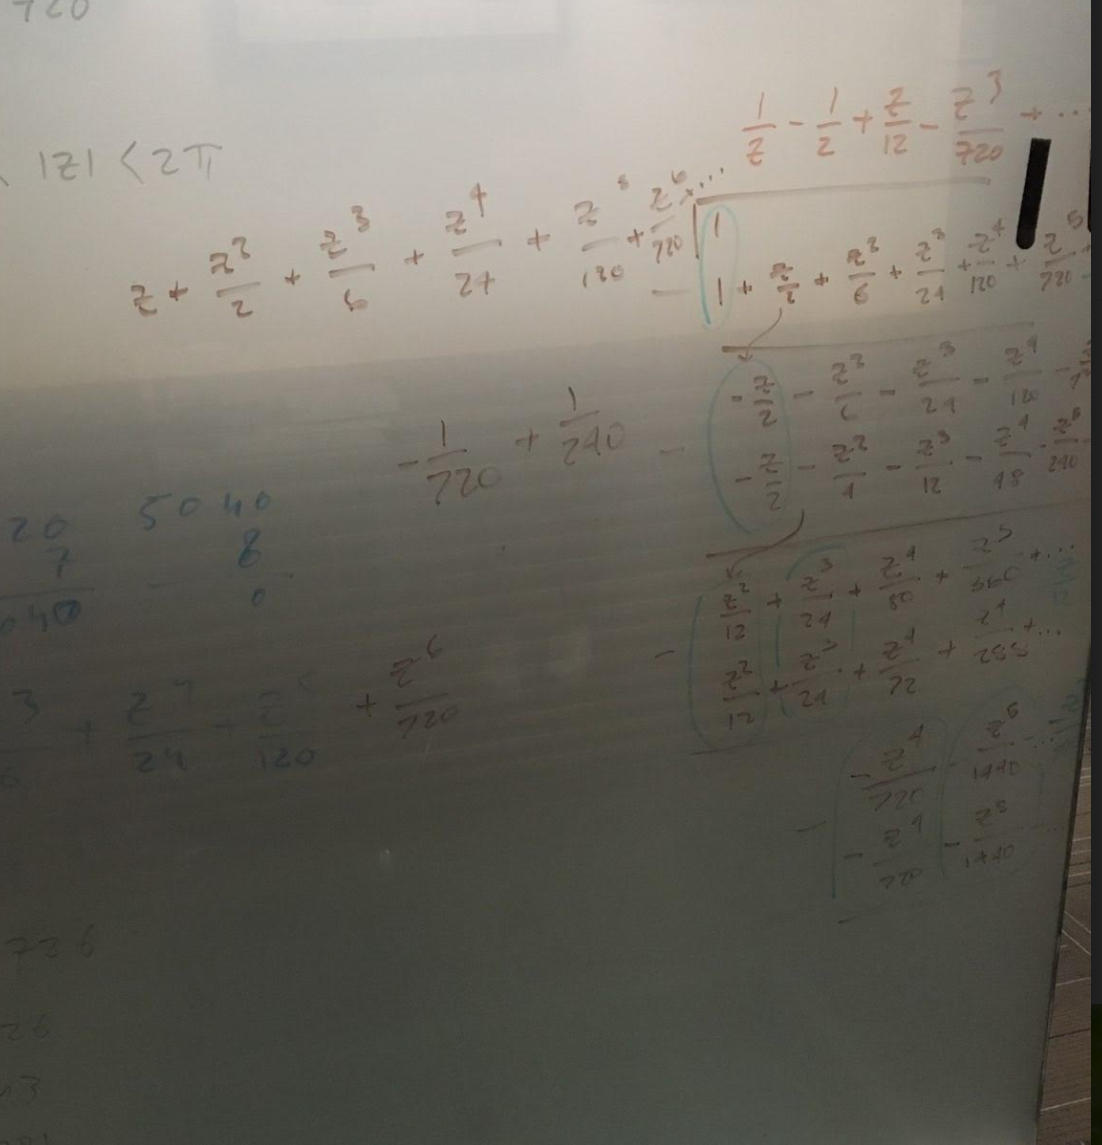
\includegraphics[scale=0.5]{long_div1.png}}
\caption{}
\label{fig}
\end{figure} \cs{A better picture might be nice...}

The derivative of the sequence doesn't exist at $z = 0$, as the denominator $e^z -1$ becomes zero. Likewise, since $e^z$ is periodic vertically ever $2\pi i$, the denominator is zero again at $z = 2\pi i$, causing the function to be undefined and the derivative to not exist. There is only one real value to make $e^z \cs{-1} = 0$, \cs{($e^z$ is never 0)} which is $z = 0$, hence the largest annulated disk centered at $0$ on which the Laurent series is valid is $0 < |z| < |2\pi i| = 2\pi$.

\cs{5/5}

\fbox{problem 9} The Euler numbers are defined to be $n$th the coefficients of the series $1/\cosh z$ multiplied by $2n!$\\
\fbox{solution} To find the Euler numbers, we first need to find the Taylor series representation of $1/\cosh z$ centered at the origin. To do this, recall the series representation for $\cosh z$, $\cosh z = \infsum z^(2n)/(2n)!$. Dividing $1$ by this series, we obtain what is shown in figure 2. There are actually no negative powers of $z$ in this series, hence it is the taylor series representation in the region in which this is defined centered at the origin. The function $\cosh{z}$ has zeros ever multiple of $\pi/2 i$ \cs{That isn't quite right -- it's at differences from $i\pi/2$ of multiples of $2\pi i$.} , as shown in the theorem of section 39 of chapter 3. Hence $1/\cosh z$ is analytic everywhere besides where it is undefined, which is at the zeros of $\cosh z$. Hence the largest possible disk throughout which $1/\cosh z$ is analytic is $|z| < \pi/2$. Hence $1/\cosh z = 1 - z^2/2 + 5/24 z^4 - 61/720z^6$. Hence, as can be seen from here, $E_n = 0$ for all odd $n$, and $E_0 = 1, E_2  = -1, E_4 = 5, E_6 = -61$.\\

\fbox{remark} There is something so amazing about integer sequences arising from representations for continuous functions. It's so mysterious.\\

\cs{5/5}

\cs{Sec 73: 10/10} 

\begin{figure}[htbp]
\centerline{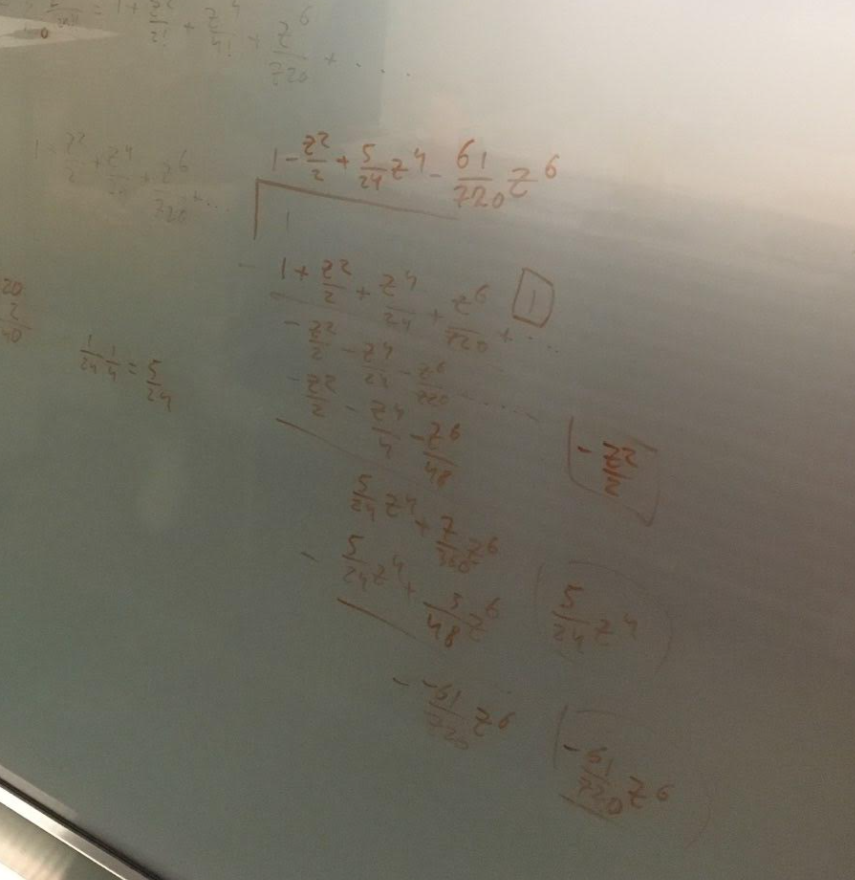
\includegraphics[scale=0.5]{long_div2.png}}
\caption{}
\label{fig}
\end{figure}




\fbox{problem 1b} Find $Res_{z = 0}z\cos(1/z)$.\\

\fbox{solution} To find the residue centered at $z = 0$, we first must find the Laurent series centered at $0$. To do this, we first substitute $1/z$ for $z$ in the taylor series $$
\cos z = \infsum (-1)^n\frac{z^{2n}}{(2n)!}:|z| < \infty\rightarrow \infsum \frac{(-1)^n}{(2n)!}z^{-2n}: 0<|z|<\infty.$$

Hence wee can substitute this into $z\cos z$ to find $z\cos z = \infsum(-1)^n/(2n)!z^{-2n +1} = z - 1/2z^{-1}+...$. The coefficient of the $-1$ power term is $-1/2$, hence the residue around $z = 0$ of $z\cos z$ is $-1/2$.\\

\cs{5/5}

\fbox{2c} Let $C$ be the curve $|z| = 1$ in the positively oriented sense, and let $f(z) = z^2 \exp(1/z)$. Find $\int_C f(z)dz$.\\
\fbox{solution} First, we need to find $1/z^2f(1/z) = 1/z^2(1/z^2\exp z) = 1/z^4 \exp z$. Using the maclaurin expansion for $\exp z$, we have \cs{a great start?} 

\cs{2/5 Let me know if you finish it.}

\\
\fbox{4b} Compute $\int_C f(z)dz$ where $f(z) = 1/(1+z^2)$ and $C$ is the circle $|z| = 2$ oriented positively.\\

\fbox{solution} Rational functions of polynomials always have a finite number of singular points in any given region, hence the region contained by $C$ has a finite number of singular points, so we can use the residue theorem. This requires that we find the laurent series expansion for $1/z^2 f(1/z) = 1/z^2(1/(1-(1/z^2))$. To find this, we can find the Laurent series expansion for $1/(1+z^2)$ using polynomial long division, and substitute $z$ for $1/z$. This will yield the series $1 - z^2 + ...$ for all $2< |z| < \infty$ (since the only singularities lie in the region enclosed by $C$). Hence we have the $1/z^2f(1/z) = 1/z^2(1 -z^2 + ...) = 1/z^2 - 1 +..$. There is no $-1$ power of $z$ term, hence the coefficient for the first negative power of $z$ is zero, and the residue around $z = 0$ of $1/z^2f(1/z) = 0$. Hence by the residue theorem it follows that the integral is zero as well.\\

\cs{5/5}

\fbox{7} I am still working on this one, it's got me stumped

\cs{Use the theorem in Section 77 and then multiply numerator and denominator by $z^{m-2}.$ Let me know if you do this one.}

\cs{Sec 77: 12/20}

\end{document}